% Compile: latexmk -pdf -interaction=nonstopmode -halt-on-error main.tex
% This document is modular: each conceptual section is a separate \input file.
\documentclass[11pt,oneside]{book}
\usepackage[T1]{fontenc}
\usepackage[utf8]{inputenc}
\usepackage{lmodern}
\usepackage[margin=1.05in,headheight=14pt]{geometry}
\usepackage{amsmath,amssymb,amsthm,mathtools,bm,mathrsfs}
\usepackage{microtype,booktabs,array,tabularx,longtable,multirow,siunitx}
\usepackage{enumitem,graphicx,xcolor,tikz,pgfplots,listings}
\usepackage[most]{tcolorbox}
\usepackage{fancyhdr}
\usepackage[hidelinks]{hyperref}
\usepackage[capitalize,nameinlink,noabbrev]{cleveref}
\usepackage{bookmark}
\usetikzlibrary{arrows.meta,positioning,calc,angles,quotes}
\pgfplotsset{compat=1.18}
\definecolor{navy}{HTML}{183353}
\definecolor{teal}{HTML}{166C7A}
\definecolor{warm}{HTML}{9D5B2E}
\definecolor{slate}{HTML}{475569}
\hypersetup{colorlinks=true,linkcolor=navy,citecolor=teal,urlcolor=teal}
\setlist[itemize]{topsep=3pt,itemsep=2pt}
\setlist[enumerate]{topsep=3pt,itemsep=3pt}
\numberwithin{equation}{chapter}
\newtheorem{theorem}{Theorem}[chapter]
\newtheorem{proposition}[theorem]{Proposition}
\newtheorem{lemma}[theorem]{Lemma}
\newtheorem{corollary}[theorem]{Corollary}
\newtheorem{definition}[theorem]{Definition}
\newtheorem{remark}[theorem]{Remark}
\newtheorem{example}[theorem]{Example}
\newtheorem{claim}[theorem]{Claim}
\newcommand{\R}{\mathbb{R}}
\newcommand{\Ssym}{\mathbb{S}}
\newcommand{\Sp}{\mathbb{S}_{+}}
\newcommand{\E}{\mathbb{E}}
\newcommand{\diag}{\operatorname{diag}}
\newcommand{\Diag}{\operatorname{Diag}}
\newcommand{\tr}{\operatorname{tr}}
\newcommand{\rank}{\operatorname{rank}}
\newcommand{\range}{\operatorname{range}}
\newcommand{\nullsp}{\operatorname{null}}
\newcommand{\OPT}{\operatorname{OPT}}
\newcommand{\Cut}{\operatorname{Cut}}
\newcommand{\ip}[2]{\left\langle #1,#2\right\rangle}
\newcommand{\norm}[1]{\left\lVert #1\right\rVert}
\newcommand{\abs}[1]{\left\lvert #1\right\rvert}
\newcommand{\one}{\boldsymbol{1}}
\newcommand{\st}{\text{subject to}}
\newtcolorbox{intuition}[1][]{colback=teal!4,colframe=teal!55!black,title=Geometric interpretation,#1}
\newtcolorbox{caution}[1][]{colback=warm!5,colframe=warm!70!black,title=Important qualification,#1}
\newtcolorbox{takeaway}[1][]{colback=navy!3,colframe=navy!45,title=Key identity,#1}
\lstdefinestyle{py}{language=Python,basicstyle=\ttfamily\footnotesize,breaklines=true,frame=single,rulecolor=\color{slate!40},numbers=left,numberstyle=\tiny\color{slate},showstringspaces=false,keywordstyle=\color{navy}\bfseries,commentstyle=\color{teal},stringstyle=\color{warm},tabsize=4}
\pagestyle{fancy}\fancyhf{}\fancyhead[L]{\small\color{slate}Max-Cut, SDP and EVA}\fancyhead[R]{\small\color{slate}\nouppercase{\leftmark}}\fancyfoot[C]{\thepage}
\setcounter{tocdepth}{2}
\title{\Huge\bfseries The Max-Cut Semidefinite Relaxation,\\[.4em] Gram Factorization, and Efficient Vector Ascent\\[.6em]\Large A Rigorous Theory-to-Examples Monograph}
\author{Independent mathematical exposition and reproducible examples\\[.3em]\normalsize Prepared for the maxkcut research project}
\date{November 2026\\\small Version 1.0 --- modular source edition}
\begin{document}
\frontmatter\maketitle
\chapter*{Preface and Reading Guide}
\addcontentsline{toc}{chapter}{Preface and Reading Guide}
This monograph develops the connection
\[
\text{discrete Max-Cut}\ \longrightarrow\ \text{convex SDP}\ \longleftrightarrow\
\text{Gram vectors}\ \longrightarrow\ \text{EVA}\ \longrightarrow\ \text{rounding}.
\]
Part I emphasizes definitions, proofs, distinctions among first-order stationarity, second-order conditions, and global optimality, and the algebra of Cholesky and spectral factorizations. Part II supplies two \emph{nontrivial, analytically solvable} examples: the frustrated five-cycle $C_5$ and a six-vertex wheel $W_6$ with a weighted spoke parameter. We exhibit their primal embeddings and positive-semidefinite dual slacks, quantify their integrality gaps, and trace the actual row-update algorithm numerically.

The primary EVA reference is Gonzalez-Torres \emph{et al.} (2026), \emph{EVA: A fast greedy optimization algorithm for the max-cut vector relaxation problem}~\cite{eva2026}. The classical SDP and rounding originate with Goemans--Williamson~\cite{gw1995}; low-rank nonconvex optimization requires additional nuance, discussed with references to Burer--Monteiro, Boumal--Voroninski--Bandeira, and Waldspurger--Waters~\cite{burer2003,boumal2016,boumal2020,waldspurger2020}. The user's earlier thesis and clustering paper provide the rounding context~\cite{rodriguez2021,rodriguez2020}. The independent example-checking script accompanies this source distribution.

\begin{caution}
Statements explicitly attributed to the EVA paper are distinguished from theorems established here. In particular, \emph{existence of an optimal low-rank Gram matrix}, \emph{first-order KKT stationarity}, and \emph{guaranteed global optimality of a particular EVA iterate} are different mathematical claims. Whenever a numerical method terminates at a finite tolerance, its primal value is not automatically a certified upper bound. A dual feasible matrix is needed for certification.
\end{caution}

\paragraph{How to edit.} Each file under \texttt{sections/} is a logical concept. Change it in isolation and retain its \verb|\input{sections/name}| in \texttt{main.tex}. The sample code is under \texttt{code/}; the entry point is \texttt{latexmk -pdf main.tex}. No external images are required.

\tableofcontents
\mainmatter
\part{Mathematical Foundations and Theoretical Analysis}
\chapter{Notation, Mathematical Objects, and Scope}\label{ch:notation}
\section{Objects, indices, and conventions}
Let $G=(V,E,w)$ be a finite, undirected, loop-free weighted graph with $V=\{1,\ldots,n\}$ and edge weights $w:E\to\R$. Write $w_{ij}=w_{ji}$ for the adjacency coefficients, with $w_{ii}=0$ and $w_{ij}=0$ for nonedges. Unless stated otherwise, sums over $E$ count each undirected edge \emph{once}; a sum over all ordered pairs counts each twice. The symbol $m=|E|$ denotes the number of edges, not the SDP number of constraints (which is $n$).

\begin{longtable}{>{\(}l<{\)}p{0.70\textwidth}}
\toprule
\text{Symbol}&\text{Meaning}\\\midrule
n,p & Number of graph vertices; embedding dimension (rank budget).\\
W & Symmetric weighted adjacency matrix in $\Ssym^n$.\\
d_i, D & Signed weighted degree $d_i=\sum_jw_{ij}$; $D=\Diag(d)$.\\
L=D-W & Weighted graph Laplacian (not necessarily PSD if weights are signed).\\
x_i\in\{-1,+1\} & Discrete side assigned to vertex $i$.\\
X\in\Ssym^n & Symmetric Gram matrix, often $X_{ij}=y_i^\top y_j$.\\
Y\in\R^{n\times p} & Matrix whose $i$th row is $y_i^\top\in\R^{1\times p}$.\\
\Ssym_+^n & Cone of real symmetric positive-semidefinite $n\times n$ matrices.\\
\ip{A}{B} & Frobenius inner product $\tr(A^\top B)=\sum_{ij}A_{ij}B_{ij}$.\\
\norm{A}_F & Frobenius norm $\sqrt{\ip{A}{A}}$.\\
\lambda_{\min}(A) & Smallest real eigenvalue of a symmetric matrix $A$.\\
\preceq,\succeq & Loewner partial order, defined by PSD differences.\\
\nu,Z & SDP dual diagonal vector and dual slack matrix.\\
h_i,s_i & EVA local field $h_i=\sum_j w_{ij}y_j$ and its length $s_i=\norm{h_i}$.\\
\bottomrule
\end{longtable}

\section{A precise objective normalization}
For unit vectors, define
\begin{equation}\label{eq:vector-objective}
F(Y)=\frac12\sum_{\{i,j\}\in E}w_{ij}(1-y_i^\top y_j).
\end{equation}
A graph cut with spins $x\in\{\pm1\}^n$ has identical normalization: $F(x)=\sum_{\{i,j\}\in E}w_{ij}\mathbb{1}[x_i\ne x_j]$. Equivalently,
\begin{equation}\label{eq:laplacian-objective}
F(X)=\frac14\ip{L}{X}\qquad \text{when }X_{ii}=1\ (1\le i\le n).
\end{equation}
The equality follows from $\ip{L}{X}=\sum_id_iX_{ii}-\sum_{ij}w_{ij}X_{ij}=\sum_{\{i,j\}\in E}2w_{ij}(1-X_{ij})$.

\begin{takeaway}
The notation $\max_XF(X)$ means \emph{choose a feasible matrix $X$ to maximize a scalar}. It does \emph{not} mean maximize each entry, the Frobenius norm, or $X$ in the Loewner partial order.
\end{takeaway}

\section{Assumptions to watch}
Nonnegative weights $w_{ij}\ge0$ are needed for the standard Goemans--Williamson $0.878\ldots$ multiplicative ratio, as presented here. The algebra of the SDP, EVA update, and primal--dual certificates also applies to signed weights, with care about negative optimum values and ratio interpretations. We use exact arithmetic in analytic theorems and explicitly distinguish it from floating-point computation in Part II.

\chapter{Discrete Max-Cut and Quadratic Optimization}\label{ch:discrete}
\section{Indicator and Ising-spin formulations}
A cut is a bipartition $V=S\sqcup (V\setminus S)$. Assign $x_i=+1$ if $i\in S$, and $x_i=-1$ otherwise. The elementary identity
\begin{equation}\label{eq:cut-indicator}
\mathbb{1}[x_i\ne x_j]=\frac{1-x_ix_j}{2}
\end{equation}
holds because $x_ix_j\in\{\pm1\}$. Thus
\begin{equation}\label{eq:iqp}
\OPT_{\mathrm{MC}}=\max_{x\in\{\pm1\}^n}\frac12\sum_{\{i,j\}\in E}w_{ij}(1-x_ix_j)=\max_{x\in\{\pm1\}^n}\frac14x^\top Lx.
\end{equation}
To verify the Laplacian formula, expand $x^\top Lx=\sum_{\{i,j\}\in E}w_{ij}(x_i-x_j)^2$, where $(x_i-x_j)^2=4$ for crossing edges and zero for noncrossing edges.

\begin{definition}[Cut polytope in Gram coordinates]
The matrix of a cut $x$ is $X=xx^\top$. The set $\mathcal Q_n=\{xx^\top:x\in\{\pm1\}^n\}$ contains every discrete cut matrix, and $\operatorname{conv}(\mathcal Q_n)$ is the convex hull of those matrices. Its entries satisfy $X_{ii}=1$, $X_{ij}\in\{\pm1\}$, $X\succeq0$, and $\rank(X)=1$.
\end{definition}
Since $xx^\top=(-x)(-x)^\top$, swapping the two sides of a cut does not change its Gram matrix. The discrete solution space has $2^{n-1}$ possible cut matrices (including the trivial cut) for $n\ge1$.

\section{Why the quadratic formulation is difficult}
The feasible set is discrete and exponential in $n$. Quadratic interactions $x_ix_j$ couple choices at different vertices: making one edge cross may prevent other edges from crossing. On an odd cycle, for example, no sign assignment can cut every edge; traversing an odd number of sign changes cannot return to the original sign. This \emph{frustration} is a source of the integrality gap exhibited in \cref{ch:cycle5,ch:wheel6}.

\section{The continuous relaxation idea}
Replace the scalar spins $x_i\in\{\pm1\}$ by unit vectors $y_i\in\R^p$. The original problem is embedded in the new one by selecting $y_i=x_ie_1$ where $e_1$ is any unit vector. Hence, for every $p\ge1$,
\begin{equation}
\OPT_{\mathrm{MC}}\le \max_{\norm{y_i}=1}F(Y)\le\OPT_{\mathrm{SDP}}.
\end{equation}
The first inequality becomes equality at $p=1$; the second becomes equality for $p=n$. The latter statement follows from Gram factorization, not from the success of a particular nonconvex solver.

\section{Statistical-mechanical interpretation}
The spins $x_i$ constitute a two-state Ising system. With zero external fields, maximizing the cut corresponds (up to an affine transformation) to minimizing an antiferromagnetic energy $H(x)=\sum_{\{i,j\}\in E}w_{ij}x_ix_j$. Replacing Ising spins by vectors produces a classical $O(p)$ spin model with spherical constraints, in which the local alignment field $h_i$ acquires the interpretation of an effective interaction field. For positive edges, the interaction is antiferromagnetic; for negative edges, it is ferromagnetic in the cut objective.

\chapter{Positive-Semidefinite Geometry, Gram Matrices, and Spectra}\label{ch:psd}
\section{The PSD cone}
\begin{definition}
A real symmetric $X\in\Ssym^n$ is \emph{positive semidefinite}, written $X\succeq0$, when $z^\top Xz\ge0$ for every $z\in\R^n$. It is positive definite, $X\succ0$, if the inequality is strict for nonzero $z$.
\end{definition}
\begin{theorem}[Equivalent PSD characterizations]\label{thm:psd-equiv}
For symmetric $X\in\Ssym^n$, the following are equivalent:
\begin{enumerate}
\item $X\succeq0$.
\item Every eigenvalue of $X$ is nonnegative.
\item $X=YY^\top$ for some real matrix $Y$.
\item $X=Q\Lambda Q^\top$ with $Q^\top Q=I$ and diagonal $\Lambda\succeq0$.
\end{enumerate}
\end{theorem}
\begin{proof}
By the spectral theorem, $X=Q\Lambda Q^\top$. With $z=Qv$, $z^\top Xz=\sum_j\lambda_jv_j^2$, which is nonnegative for all $v$ exactly when every $\lambda_j\ge0$. Then $Y=Q\Lambda^{1/2}$ yields $YY^\top=X$. Conversely, $z^\top YY^\top z=\norm{Y^\top z}^2\ge0$.
\end{proof}

\section{The elliptope and its geometry}
\begin{definition}[Elliptope]
The real correlation elliptope is
\[
\mathcal E_n=\{X\in\Ssym_+^n:\diag(X)=\one\}.
\]
Every $X\in\mathcal E_n$ is a Gram matrix of unit vectors $y_1,\ldots,y_n$.
\end{definition}
Each two-by-two principal minor is nonnegative, so $1-X_{ij}^2\ge0$; hence $-1\le X_{ij}\le1$. However, the entries are \emph{globally coupled}: satisfying all pairwise bounds is insufficient for PSD, because all principal minors and spectral conditions must be compatible.

\begin{lemma}[Metric induced by the Gram matrix]\label{lem:gram-distance}
For $\norm{y_i}=\norm{y_j}=1$,
\[
\norm{y_i-y_j}^2=2(1-X_{ij}),\qquad X_{ij}=\cos\theta_{ij}.
\]
\end{lemma}
\begin{proof}
Expand $\norm{y_i-y_j}^2=\norm{y_i}^2+\norm{y_j}^2-2y_i^\top y_j$ and use the definition of the angle between unit vectors.
\end{proof}
\begin{intuition}
Maximizing $F(X)$ for positive weights tends to push vectors on heavily weighted edges far apart on a sphere; it does not require every pair of vectors to be antipodal, which may be geometrically impossible on odd cycles. The objective is a weighted sum of squared chord distances:
\[
F(Y)=\frac14\sum_{\{i,j\}\in E}w_{ij}\norm{y_i-y_j}^2.
\]
\end{intuition}

\section{Partial order is not an entrywise objective}
The Loewner order $A\succeq B$ means $A-B\succeq0$, not $A_{ij}\ge B_{ij}$. It is not a total order. For unit-diagonal feasible matrices $X,X'$, $X\succeq X'$ actually forces $X=X'$: the PSD difference $H=X-X'$ has diagonal zero; a PSD matrix with zero diagonal is zero, by $|H_{ij}|^2\le H_{ii}H_{jj}=0$. Thus, \emph{maximize a PSD matrix} is not what the SDP does. Instead it maximizes the \emph{linear functional} $\ip{C}{X}$.

\section{Spectral and trace tools}
For symmetric $C$ and PSD $X$, $\ip{C}{X}=\tr(CX)$; the sign need not be nonnegative unless $C\succeq0$. A useful upper bound for nonnegative-weight graph Laplacians is
\begin{equation}\label{eq:spectral-bound}
F(X)=\frac14\tr(LX)\le \frac14\lambda_{\max}(L)\tr(X)=\frac n4\lambda_{\max}(L),
\end{equation}
because $L\preceq\lambda_{\max}(L)I$ and $X\succeq0$. This is usually not sharp; primal--dual certificates will produce sharper bounds in Part II.

\chapter{The Convex Max-Cut SDP: Derivation and Exactness Questions}\label{ch:sdp}
\section{Lifting a quadratic program}
Introduce $X=xx^\top$ into the integer formulation \eqref{eq:iqp}. Then $x_i^2=1$ becomes $X_{ii}=1$, and $X\succeq0$ follows automatically. The condition $\rank(X)=1$ remains nonconvex. Dropping that condition yields
\begin{equation}\label{eq:sdp-primal}
\boxed{\begin{aligned}
\OPT_{\mathrm{SDP}}=\max_{X\in\Ssym^n}\quad &\ip{C}{X},\qquad C:=\frac14L,\\
\st\quad&\diag(X)=\one,\\
&X\succeq0.
\end{aligned}}
\end{equation}
The objective is linear in $X$, and the feasible region is a convex compact spectrahedron. Optimization is therefore a \emph{convex optimization problem} in the standard sense (maximization of a concave---here linear---function over a convex set).

\begin{proposition}[Relaxation and upper bound]\label{prop:upper}
For any weighted undirected graph,
\[
\OPT_{\mathrm{MC}}\le\OPT_{\mathrm{SDP}}.
\]
\end{proposition}
\begin{proof}
Given $x\in\{\pm1\}^n$, $X=xx^\top$ is SDP-feasible and $\ip{C}{X}=\frac14x^\top Lx$. Thus the SDP feasible region includes every discrete cut matrix and can only attain a greater or equal maximum.
\end{proof}

\section{The vector program}
Replacing $X$ by $YY^\top$ gives
\begin{equation}\label{eq:bm}
\boxed{\max_{Y\in\R^{n\times p}}\ \tr(Y^\top CY)\quad \st\quad \norm{y_i}=1\quad\forall i.}
\end{equation}
For $p=n$, \cref{thm:psd-equiv} implies this parameterization is globally equivalent to \eqref{eq:sdp-primal}: every feasible $X$ admits a factor. For $p<n$ it covers only the matrices in $\mathcal E_n$ with rank at most $p$. The nonconvexity is in the factorized constraint surface, not in the original SDP.

\section{Slater's condition and compactness}
The identity $I_n$ satisfies $\diag(I_n)=\one$ and $I_n\succ0$, so strict feasibility holds. The feasible set is closed and bounded ($|X_{ij}|\le1$), hence compact. Therefore an optimal $X^*$ exists, and SDP strong duality applies. The use of an interior-point method, first-order conic solver, or ADMM affects numerical accuracy and computational resources, but not the mathematical program being solved.

\section{Why rank one is special}
If a feasible $X$ has rank one, write $X=vv^\top$. Then $1=X_{ii}=v_i^2$, so $v_i\in\{\pm1\}$. Thus any rank-one SDP solution gives an exact discrete cut. Conversely, every discrete cut matrix has rank one. If the SDP optimizer has rank greater than one, \emph{rounding} is required to recover spins, though higher-rank optimal matrices may coexist with rank-one optimal matrices as in the complete graph $K_4$.

\section{Rank-restricted SDPs are not the same feasible set}
A rank bound such as $p\approx\sqrt{2n}$ has an existential interpretation: for an SDP with $n$ affine equality constraints there is an \emph{optimal solution} of sufficiently low rank. It does not imply every $X\in\mathcal E_n$ admits a $p$-column factor. For example, $I_n\in\mathcal E_n$ has rank $n$. See \cref{ch:rank} for precise rank claims and algorithmic cautions.

\chapter{Conic Duality, KKT Conditions, and Optimality Certificates}\label{ch:dual}
\section{Deriving the SDP dual from the Lagrangian}
For \eqref{eq:sdp-primal}, set $C=L/4$ and introduce multipliers $\nu\in\R^n$ for the constraints $X_{ii}=1$. The maximization Lagrangian is
\begin{align}
\mathcal L(X,\nu)&=\ip{C}{X}+\sum_i\nu_i(1-X_{ii})\\
&=\one^\top\nu+\ip{C-\Diag(\nu)}{X}.
\end{align}
For the supremum of $\mathcal L$ over $X\succeq0$ to be finite, we require $C-\Diag(\nu)\preceq0$. Otherwise a positive-eigenvalue direction can be scaled to make the supremum infinite. Hence the dual is
\begin{equation}\label{eq:sdp-dual}
\boxed{\begin{aligned}
\min_{\nu\in\R^n}\quad &\sum_{i=1}^n\nu_i\\
\st\quad &Z:=\Diag(\nu)-C\succeq0.
\end{aligned}}
\end{equation}
The matrix $Z$ is the \emph{dual slack}. Unlike a feasible primal matrix, which gives a lower bound on the SDP maximum, any dual-feasible $\nu$ gives an upper bound.

\begin{theorem}[Weak duality]\label{thm:weak}
If $X\succeq0$, $\diag(X)=\one$ and $Z=\Diag(\nu)-C\succeq0$, then
\[
\ip{C}{X}\le\one^\top\nu.
\]
\end{theorem}
\begin{proof}
The gap is $\one^\top\nu-\ip{C}{X}=\ip{\Diag(\nu)-C}{X}=\ip{Z}{X}\ge0$, since the trace of a product of two PSD matrices is nonnegative: $\tr(ZX)=\tr(X^{1/2}ZX^{1/2})\ge0$.
\end{proof}

\begin{theorem}[Strong duality and complementary slackness]\label{thm:strong}
The Max-Cut SDP has equal attained primal and dual optimal values. A feasible pair $(X,\nu)$ is optimal if and only if
\begin{equation}\label{eq:complementarity}
\ip{Z}{X}=0,\qquad Z=\Diag(\nu)-C\succeq0.
\end{equation}
For PSD $X,Z$, zero trace product implies $ZX=XZ=0$.
\end{theorem}
\begin{proof}
Strict primal feasibility holds at $I_n$, so conic Slater duality gives equal values and attainment. Weak duality proves sufficiency of zero gap. For the final claim, $\tr(ZX)=\norm{Z^{1/2}X^{1/2}}_F^2=0$ forces $Z^{1/2}X^{1/2}=0$ and hence $ZX=XZ=0$.
\end{proof}

\section{Exact and approximate certificates}
A certificate is \emph{exact} when $X$ and $Z$ are exactly PSD, $\diag X=\one$, and $\ip{Z}{X}=0$. For floating-point output, report all of
\begin{equation}
\norm{\diag(X)-\one}_\infty,\quad-\lambda_{\min}(X),\quad-\lambda_{\min}(Z),\quad\abs{\ip{Z}{X}},\quad\one^\top\nu-\ip{C}{X}.
\end{equation}
Clipping a tiny negative eigenvalue in the primal matrix may repair PSD but also alter the diagonal and objective; the postprocessed matrix must be inspected separately.

\section{KKT equations for factorized coordinates}
For $Y\in\R^{n\times p}$ with $\norm{y_i}=1$, define
\[
\mathscr L(Y,\nu)=\tr(Y^\top CY)-\sum_i\nu_i(\norm{y_i}^2-1).
\]
The Euclidean gradient with respect to $Y$ is
\[
\nabla_Y\mathscr L=2(C-\Diag(\nu))Y=-2ZY.
\]
Thus the first-order KKT stationarity equations are
\begin{equation}\label{eq:factor-kkt}
ZY=0,\quad \norm{y_i}=1\ (i=1,\ldots,n).
\end{equation}
Crucially, \emph{factor KKT stationarity alone does not guarantee $Z\succeq0$}. It is the missing dual inequality that separates a generic stationary embedding from a certified global SDP solution.

\section{Second-order KKT geometry}
A tangent perturbation $U\in\R^{n\times p}$ to the product of spheres satisfies $u_i^\top y_i=0$ for each row $i$. At a local maximum, the Hessian of the constrained Lagrangian is negative semidefinite on these tangent directions, yielding
\begin{equation}\label{eq:second-order}
\tr(U^\top ZU)\ge0\qquad \text{for every tangent }U.
\end{equation}
This condition is weaker than $Z\succeq0$ in general, because tangent variations do not cover all directions in $\R^{n\times p}$. A rank-deficient factor supplies a particularly useful class of tangent variations, as proved in \cref{ch:rank}.

\chapter{Cholesky, Spectral Factorization, and Numerical Rank}\label{ch:factorization}
\section{A square root of a Gram matrix is not another optimizer}
Given an SDP solution $X\succeq0$, a matrix $Y$ satisfying $YY^\top=X$ represents a configuration of vectors with exactly the inner products encoded in $X$. Computing $Y$ after an SDP solve is \emph{linear algebraic factorization}; it does not improve or reoptimize the SDP objective.

\section{Cholesky factorization}
\begin{theorem}[Cholesky for positive-definite matrices]
If $X\in\Ssym_{++}^n$, then there is a unique lower-triangular $L_c$ with strictly positive diagonal entries such that $X=L_cL_c^\top$.
\end{theorem}
The matrix $L_c$ has $n$ rows; row $i$ is a coordinate vector for graph vertex $i$. Beware that we write $L_c$ for the Cholesky factor, reserving $L=D-W$ for the graph Laplacian. These are unrelated matrices.

\paragraph{Why Cholesky may fail at the SDP optimum.} A positive-semidefinite matrix can be singular (zero eigenvalues). A standard numerical Cholesky routine is designed for positive-definite input and can fail on singular matrices. Many Max-Cut SDP optima are deliberately low rank: the exact embeddings in \cref{ch:cycle5,ch:wheel6} have ranks two and three. Adding a ``jitter'' term $\delta I$ makes Cholesky possible but changes the matrix, diagonal, objective, and sometimes the rounded-cut distribution. It must not silently replace the original SDP solution.

\section{Spectral factorization}
Let $X=Q\Lambda Q^\top$ with $\Lambda=\Diag(\lambda_1,\ldots,\lambda_n)$ and $\lambda_j\ge0$. Then
\begin{equation}\label{eq:eigfactor}
Y=Q_{:,I}\Diag(\sqrt{\lambda_j}:j\in I),\quad I=\{j:\lambda_j>0\},\qquad YY^\top=X.
\end{equation}
This yields a \emph{thin} factor with $p=\rank(X)$ columns and avoids requiring positive definiteness. The columns of $Y$ are scaled eigenvectors, but its \emph{rows} are the graph-vertex embeddings. Confusing rows with columns changes the dimensional interpretation.

\section{Numerical PSD projection and renormalization}
A first-order conic solver may return an approximately symmetric matrix $\widehat X$ with small negative eigenvalues. One common repair is
\[
S=\tfrac12(\widehat X+\widehat X^\top)=Q\Lambda Q^\top,\quad
\widetilde X=Q\Diag(\max\{\lambda_j,0\})Q^\top.
\]
This is the Frobenius-nearest positive-semidefinite matrix to $S$ in the unweighted Euclidean metric. If $\diag(\widetilde X)\ne\one$, create row vectors $y_i$ from the spectral square root and normalize them:
\[
\widehat y_i=\frac{y_i}{\norm{y_i}},\qquad
\widehat X_{ij}=\frac{\widetilde X_{ij}}{\sqrt{\widetilde X_{ii}\widetilde X_{jj}}}.
\]
This gives another feasible Max-Cut elliptope matrix if no denominator vanishes, but need not preserve the original objective. This is the approach used by the project's \texttt{rounding.factorize} implementation, rather than ordinary Cholesky.

\section{Orthogonal invariance and identifiability}
If $R\in\R^{p\times p}$ is orthogonal, then
\[
(YR)(YR)^\top=YRR^\top Y^\top=YY^\top.
\]
Thus the coordinate vectors are not uniquely identifiable: rotating or reflecting the entire configuration changes $Y$ but not $X$ or the graph objective. Conversely, for two full-column-rank minimal factors of the same Gram matrix, there exists an orthogonal change of coordinates relating them. Compare embeddings by \emph{Gram matrices} or orthogonally aligned factors, not by unaligned entries.

\section{SVD and rank diagnostics}
If $Y=U\Sigma V^\top$ is a compact singular-value decomposition, then $YY^\top=U\Sigma^2U^\top$. Its nonzero eigenvalues are the squared singular values of $Y$. Defining numerical rank requires a declared tolerance $\tau$; e.g., count $\lambda_j>\tau\lambda_{\max}$. A small eigenvalue can carry genuine geometric information, so arbitrary truncation must be treated as a separate experiment.

\chapter{Goemans--Williamson Rounding and Approximation Theory}\label{ch:rounding}
\section{Random hyperplanes}
Given unit vectors $y_1,\ldots,y_n\in\R^p$ and a rotationally invariant random normal vector $g\sim N(0,I_p)$, define
\begin{equation}\label{eq:gw-round}
x_i=\operatorname{sign}(y_i^\top g).
\end{equation}
The side of the hyperplane orthogonal to $g$ determines the cut. Because a Gaussian is rotationally invariant, only pairwise angles matter.

\begin{lemma}[Separation probability]\label{lem:sep}
If $\theta_{ij}=\arccos(y_i^\top y_j)\in[0,\pi]$, then
\[
\Pr(x_i\ne x_j)=\frac{\theta_{ij}}{\pi}.
\]
\end{lemma}
\begin{proof}
Orthogonally project $g$ onto the two-dimensional plane spanned by $y_i,y_j$. Its angular direction is uniform on the circle. The signs differ precisely when the separating line's normal lies in the two wedges of total angular measure $2\theta_{ij}$ out of $2\pi$.
\end{proof}

\begin{theorem}[Goemans--Williamson performance guarantee]\label{thm:gw}
For nonnegative edge weights and an optimal SDP embedding,
\[
\E[\Cut(x)]\ge \alpha_{\mathrm{GW}}\,\OPT_{\mathrm{SDP}}\ge\alpha_{\mathrm{GW}}\,\OPT_{\mathrm{MC}},
\]
where
\begin{equation}\label{eq:alpha}
\alpha_{\mathrm{GW}}=\min_{0\le\theta\le\pi}
\frac{2\theta}{\pi(1-\cos\theta)}\approx0.878567.
\end{equation}
\end{theorem}
\begin{proof}
Linearity of expectation and \cref{lem:sep} give
$\E[\Cut(x)]=\sum_{\{i,j\}\in E}w_{ij}\theta_{ij}/\pi$. The SDP value is $\sum w_{ij}(1-\cos\theta_{ij})/2$. By the defining lower bound for $\alpha_{\mathrm{GW}}$, $\theta/\pi\ge\alpha_{\mathrm{GW}}(1-\cos\theta)/2$ for each edge. Multiply by $w_{ij}\ge0$, sum, and invoke \cref{prop:upper}.
\end{proof}

\begin{caution}
The last theorem is about the \emph{expected cut from an optimal SDP solution} with \emph{nonnegative} weights. A finite-tolerance EVA point is not automatically optimal. Signed weights invalidate the edge-by-edge nonnegative multiplication used in the guarantee. The theorem also says nothing about an individual random draw being at least $0.878\,\OPT$.
\end{caution}

\section{Probability is determined by the Gram matrix}
Even if Cholesky and spectral factors have different coordinates, they generate the same randomized-cut law under isotropic Gaussian rounding whenever they have the same Gram matrix. In particular, each pair's crossing probability is $\arccos(X_{ij})/\pi$. The joint distribution of the Gaussian projections is also determined by $X$, because $(y_i^\top g)_{i=1}^n$ is a centered Gaussian with covariance $YY^\top=X$.

\section{Clustering as a different rounder}
Rodriguez-Fernandez \emph{et al.}~\cite{rodriguez2020} replace a single random hyperplane by clustering the SDP vectors. Spherical $k$-means, antipodal initialization, medoids, and local-search improvements are empirically effective, but optimizing within-cluster distortion is not the same as maximizing the graph-cut objective. To compare rounders, \emph{hold the input Gram factor fixed}. Comparing rounders applied to different SDP factors confounds factor quality with rounding quality.

\chapter{Burer--Monteiro Geometry, Rank Bounds, and Spurious Optima}\label{ch:rank}
\section{Dimension reduction and its price}
The full SDP has $n(n+1)/2$ symmetric scalar matrix entries (with $n$ fixed diagonal constraints). A factor $Y\in\R^{n\times p}$ has $np$ scalar entries and lies on the compact manifold
\[
\mathcal M_p=(S^{p-1})^n=\{Y:\norm{y_i}=1,\ i=1,\ldots,n\}.
\]
Its dimension is $n(p-1)$, since each sphere contributes $p-1$ degrees of freedom. The factorization automatically enforces PSD, but creates nonconvexity and rotational gauge redundancy $Y\sim YR$ for $R\in O(p)$.

\section{Existential low-rank theorem}
\begin{theorem}[Extreme-point rank bound]\label{thm:rankbound}
For the Max-Cut elliptope, an SDP optimum exists with rank $r$ satisfying
\[
\frac{r(r+1)}2\le n.
\]
Consequently a factor with $p\ge\lfloor(\sqrt{8n+1}-1)/2\rfloor$ columns can represent \emph{some} SDP optimum.
\end{theorem}
\begin{proof}[Proof sketch with the essential dimension argument]
A linear function attains its optimum at an extreme point of the compact elliptope. Let $X=UU^\top$ be an extreme point of rank $r$, where $U\in\R^{n\times r}$ has full column rank. Any symmetric perturbation $H\in\Ssym^r$ induces a matrix perturbation $UHU^\top$. Requiring its diagonal to remain zero imposes $n$ homogeneous linear equations in the $r(r+1)/2$ entries of $H$. If $r(r+1)/2>n$, a nonzero $H$ exists. For sufficiently small $t>0$, both $I_r\pm tH\succeq0$, and hence $X\pm tUHU^\top$ are distinct feasible matrices averaging to $X$, contradicting extremality.
\end{proof}

\begin{remark}
The EVA reference uses a conservative rank prescription $p=\lceil\sqrt{2(n+1)}\rceil$. This is of the same order as the extreme-point bound and is large enough to \emph{represent an optimum}. It is not a claim that every full-rank feasible $X$ lies in the restricted factorization. Moreover, the ability to represent an optimum must not be mistaken for a proof that a particular sequence of coordinate updates finds it.
\end{remark}

\section{A deterministic global-optimality theorem for rank-deficient factors}
\begin{theorem}[Rank-deficient second-order point is globally SDP-optimal]\label{thm:rankdef}
Let $Y\in\mathcal M_p$ satisfy first-order stationarity and the second-order necessary condition \eqref{eq:second-order}. If $\rank(Y)<p$, then $X=YY^\top$ is globally optimal for the SDP.
\end{theorem}
\begin{proof}
Stationarity gives $ZY=0$ with $Z=\Diag(\nu)-C$. Since $\rank(Y)<p$, choose nonzero $q\in\R^p$ such that $Yq=0$. For arbitrary $z\in\R^n$, set $U=zq^\top$. Each row satisfies $u_i^\top y_i=z_iq^\top y_i=0$, so $U$ is tangent. Second-order necessity gives $0\le\tr(U^\top ZU)=\norm{q}^2z^\top Zz$. As $z$ is arbitrary, $Z\succeq0$. Thus $\nu$ is dual feasible and $ZY=0$ implies $ZX=0$. By \cref{thm:strong}, $X$ is globally SDP-optimal.
\end{proof}

\section{What generic no-spurious-optima theorems actually say}
Research on the Burer--Monteiro factorization establishes global-optimality conclusions for second-order critical points under appropriate rank and regularity assumptions; important results apply to \emph{generic} objective matrices rather than arbitrary structured graphs~\cite{boumal2016,boumal2020}. There are also counterexamples below critical rank thresholds~\cite{waldspurger2020}. The conclusions depend on which assumptions hold: stationarity order, cost genericity, constraint regularity, rank, and whether a sequence actually reaches a second-order point.

\begin{caution}
The 2026 EVA paper states a global-optimality result for sufficiently large $p$, invoking prior low-rank SDP theory. A rigorous independent audit must check the cited theorem's hypotheses and whether EVA's convergence notion is sufficient. It is mathematically unsafe to replace ``there exists a low-rank SDP optimum'' or ``the update reaches an approximate KKT point'' with ``every stopped EVA run is globally optimal.'' We use directly verifiable dual certificates whenever claiming global optimality.
\end{caution}

\chapter{EVA from First Principles: Exact Vector-Coordinate Ascent}\label{ch:eva}
\section{The optimization problem and the local field}
Efficient Vector Ascent (EVA)~\cite{eva2026} operates directly on
\begin{equation}\label{eq:eva-problem}
\max_{Y\in\mathcal M_p}F(Y)=\frac12\sum_{\{i,j\}\in E}w_{ij}(1-y_i^\top y_j),\qquad \mathcal M_p=(S^{p-1})^n.
\end{equation}
One \emph{coordinate block} is an entire vector $y_i\in\R^p$, rather than one scalar component or one entry of the Gram matrix. A sweep visits all vertices, typically in a fixed order. Within a sweep, updates use the already-updated latest rows (Gauss--Seidel, not a simultaneous Jacobi step).

Fix all vectors except $y_i$. Group the objective by edges incident to vertex $i$:
\begin{align}
F(Y)&=\underbrace{\frac12\sum_{\{a,b\}\in E,\,i\notin\{a,b\}}w_{ab}(1-y_a^\top y_b)+\frac12\sum_{j\in N(i)}w_{ij}}_{C_i\ \text{independent of }y_i}
-\frac12\sum_{j\in N(i)}w_{ij}y_i^\top y_j\\
&=C_i-\frac12 y_i^\top h_i,\qquad h_i:=\sum_{j\in N(i)}w_{ij}y_j.\label{eq:field-decomp}
\end{align}
Note that $h_i$ depends on the \emph{other} rows, so it is fixed during this individual update, even though it changes later as other vertices move. For signed $w_{ij}$, the same decomposition is valid; negative-weight edges push the local effective field in the opposite direction.

\section{Solving the spherical subproblem exactly}
The subproblem is
\begin{equation}\label{eq:local-sub}
\max_{\norm{y_i}=1}\{C_i-\tfrac12y_i^\top h_i\}\quad\Longleftrightarrow\quad\min_{\norm{y_i}=1}y_i^\top h_i.
\end{equation}
Cauchy--Schwarz says $|y_i^\top h_i|\le\norm{y_i}\norm{h_i}=\norm{h_i}$, hence $y_i^\top h_i\ge-\norm{h_i}$. If $h_i\ne0$, equality holds precisely at the negative normalized field:
\begin{equation}\label{eq:eva-update}
\boxed{y_i^{+}=-\frac{h_i}{\norm{h_i}},\qquad h_i\ne0.}
\end{equation}
Alternatively use a Lagrange multiplier: minimize $y_i^\top h_i+\frac\mu2(\norm{y_i}^2-1)$. Stationarity gives $h_i+\mu y_i=0$, so $y_i=-h_i/\mu$ and the norm constraint implies $|\mu|=\norm{h_i}$. The minimizing choice has $\mu=\norm{h_i}$; the other stationary point is the maximizer of the dot product (the worst possible coordinate choice for $F$).

\begin{definition}[Zero local field]
If $h_i=0$, the local function $C_i-\tfrac12y_i^\top h_i$ is constant on the sphere: \emph{every} unit vector is coordinate-optimal. An implementation must specify a tie policy (retain the current row, choose a deterministic tie-break, or draw a random unit row). A random tie-break can change later trajectories without changing the immediate objective.
\end{definition}

\section{Exact improvement identity and angular interpretation}
Let $s_i=\norm{h_i}>0$ and let $\theta_i=\arccos((y_i^-)^\top y_i^+)\in[0,\pi]$ be the angle between old and newly optimal row. Since $h_i=-s_iy_i^+$,
\[
(y_i^-)^\top h_i=-s_i\cos\theta_i,\qquad (y_i^+)^\top h_i=-s_i.
\]
Therefore, the exact improvement attributable to the update is
\begin{equation}\label{eq:eva-gain}
\boxed{\Delta_i=F(Y^+)-F(Y^-)=\frac{s_i}{2}(1-\cos\theta_i)=s_i\sin^2\frac{\theta_i}{2}\ge0.}
\end{equation}
This equation proves \emph{monotonic ascent} without line search or Lipschitz constants. It also explains why a small update angle often means a small objective increment, but the reverse need not hold if the local field $s_i$ is very small.

\begin{intuition}
A vector is moved to the antipodal point relative to the weighted vector sum of its neighbors. This is \emph{not} the claim that it is antipodal to each neighbor separately; such a configuration may be impossible. The update solves one local spherical optimization problem exactly.
\end{intuition}

\section{One-epoch pseudocode and cost}
\begin{tcolorbox}[colback=navy!2,colframe=navy!45,title=EVA with sequential in-place updates]
\begin{enumerate}
\item Choose $p$, initial unit rows $y_i$, maximum sweeps, and angular tolerance $\varepsilon>0$.
\item For $i=1,\ldots,n$, compute $h_i=\sum_{j\in N(i)}w_{ij}y_j$ using current rows.
\item If $h_i\ne0$, set $y_i\gets-h_i/\norm{h_i}$; otherwise follow the declared tie rule.
\item Record $\theta_i=\arccos(\operatorname{clip}((y_i^{\mathrm{old}})^\top y_i,-1,1))$.
\item Stop a sweep when $\max_i\theta_i\le\varepsilon$; otherwise continue.
\end{enumerate}
\end{tcolorbox}
The local field for vertex $i$ costs $O(\deg(i)p)$ arithmetic operations for sparse $W$. A complete sweep costs $O(mp+np)$ (usually abbreviated $O(mp)$ when the graph has no isolated vertices and $m=\Omega(n)$); storing rows and sparse graph data costs $O(np+m)$. The paper's complexity statements concern sparse graph access, not formation of a dense $n\times n$ Gram matrix, which is unnecessary for the update.

\section{Why simultaneous updates are different}
If all $h_i$ are computed from the same old $Y$ and all rows are updated simultaneously, the exact single-row monotonicity argument no longer telescopes: modifying $y_i$ changes the terms coupled to other modified rows. Thus the sequential Gauss--Seidel implementation and its monotonicity proof cannot be transferred automatically to a GPU Jacobi update. Parallel execution requires either a new proof or careful independent-set scheduling.

\chapter{Convergence, Riemannian Stationarity, and Rate Claims}\label{ch:convergence}
\section{Why the objective sequence converges}
The feasible set $\mathcal M_p$ is compact, $F$ is continuous, and every exact EVA coordinate update makes $F$ nondecreasing by \eqref{eq:eva-gain}. Consequently, for the sequential states $Y^t$,
\[
F(Y^0)\le F(Y^1)\le\cdots\le \max_{\mathcal M_p}F<\infty.
\]
The monotone convergence theorem for real sequences therefore gives $F(Y^t)\to F_\infty$. More precisely, the nonnegative coordinate gains sum to at most the finite available objective improvement:
\begin{equation}\label{eq:gain-telescope}
\sum_{t,i}\Delta_{t,i}=F_\infty-F(Y^0)<\infty\quad\Longrightarrow\quad\Delta_{t,i}\to0.
\end{equation}
This does \emph{not} immediately show that $Y^t$ converges as a matrix or that every $\theta_{t,i}\to0$. Zero fields can permit large row changes with zero gain, and symmetries can produce multiple equivalent factor representations.

\section{The product of spheres as a Riemannian manifold}
At $Y\in\mathcal M_p$, the tangent space is
\[
T_Y\mathcal M_p=\{U\in\R^{n\times p}:u_i^\top y_i=0\ \forall i\}.
\]
For the objective $F(Y)$, differentiating with respect to $y_i$ gives
\[
\nabla_{y_i}F=-\tfrac12h_i.
\]
The tangent-space orthogonal projection is $P_{y_i}z=z-(y_i^\top z)y_i$. Hence the \emph{Riemannian gradient} is
\begin{equation}\label{eq:riemgrad}
\operatorname{grad}_{y_i}F=-\frac12\left[h_i-(y_i^\top h_i)y_i\right].
\end{equation}
A stationary point of the constrained smooth problem has $h_i$ parallel to $y_i$ for every $i$. This includes both \emph{antiparallel} alignment (coordinate maximum) and \emph{parallel} alignment (coordinate minimum), so first-order Riemannian stationarity is weaker than coordinate-wise maximality. A true EVA fixed point with all $h_i\ne0$ obeys $h_i=-s_iy_i$ and is coordinate-wise maximal.

\section{Field length, gain, and angular complexity}
\begin{proposition}[Conditional $O(\varepsilon^{-2})$ sweep bound]\label{prop:conditional-rate}
Suppose every local field encountered after some initialization satisfies $s_{t,i}\ge\delta>0$, and define $B=\sup_{Y\in\mathcal M_p}F(Y)$. Then the number of \emph{sweeps} containing an update with angle $\theta_{t,i}>\varepsilon$ is at most
\[
\frac{\pi^2(B-F(Y^0))}{\delta\varepsilon^2}.
\]
\end{proposition}
\begin{proof}
For $0\le\theta\le\pi$, $1-\cos\theta=2\sin^2(\theta/2)\ge2\theta^2/\pi^2$, using the concavity lower bound $\sin u\ge2u/\pi$ on $[0,\pi/2]$. By \eqref{eq:eva-gain}, an update with $\theta>\varepsilon$ improves the objective by at least $\delta\varepsilon^2/\pi^2$. Distinct such sweeps contribute distinct positive gains, and their sum cannot exceed $B-F(Y^0)$.
\end{proof}

\begin{caution}
The uniform field lower bound is a real hypothesis, not an algebraic identity. If $h_i=0$ or $s_i\downarrow0$, small improvement alone does not control the update angle. The EVA article states an $O(\varepsilon^{-2})$ convergence result for an angular approximate-KKT criterion using additional arguments on nonvanishing fields~\cite{eva2026}. Our proposition provides a directly checkable version and makes the missing denominator issue explicit. It is not presented as a replacement for the paper's full proof.
\end{caution}

\section{What converges, and in what sense?}
Several statements should be distinguished:
\begin{enumerate}
\item \emph{Objective convergence:} $F(Y^t)\to F_\infty$, established by monotonicity and boundedness.
\item \emph{Vanishing coordinate gains:} $\Delta_{t,i}\to0$, established by summability.
\item \emph{Angular stationarity:} $\max_i\theta_{t,i}\to0$, requiring control of zero or small local fields.
\item \emph{First-order KKT:} $\operatorname{grad}F(Y^*)=0$ at an accumulation point, requiring an appropriate continuity and update-rule argument.
\item \emph{Second-order stationarity:} the constrained Hessian is negative semidefinite on all tangent directions; not implied solely by small angular moves.
\item \emph{Global SDP optimality:} needs additional rank/regularity hypotheses or a feasible dual certificate $Z\succeq0$.
\end{enumerate}
These are logically different results. Reporting one as another obscures what the numerical algorithm actually establishes.

\section{Floating-point stopping criteria}
A direct computation $\theta=\arccos(y_{\mathrm{old}}^\top y_{\mathrm{new}})$ is poorly conditioned near $\theta=0$ because $\arccos'(t)=-1/\sqrt{1-t^2}$. In double precision, rounding of a dot product near $1$ can produce an apparent angle near $10^{-8}$ radians, or zero, depending on summation order. Always clip the dot product to $[-1,1]$, report the tolerance, and do not equate tiny differences in sweep counts with different mathematical solutions.

\chapter{Reconstructing a Global-Optimality Certificate from EVA}\label{ch:certificate}
\section{From local fields to a dual candidate}
Assume $Y\in\mathcal M_p$ is a coordinate-wise EVA fixed point with each $h_i=-s_iy_i$, $s_i=\norm{h_i}\ge0$. Since the Laplacian satisfies $(LY)_i=d_iy_i-h_i=(d_i+s_i)y_i$, define
\begin{equation}\label{eq:eva-nu}
\boxed{\nu_i:=\frac{d_i+s_i}{4}.}
\end{equation}
Let
\begin{equation}\label{eq:eva-slack}
\boxed{Z:=\Diag(\nu)-\frac14L.}
\end{equation}
Then row by row $(ZY)_i=\nu_i y_i-\frac14(d_i+s_i)y_i=0$, so \emph{stationarity/complementarity} holds.

\begin{theorem}[EVA dual PSD test]\label{thm:eva-cert}
If the $Y$ above has unit rows and $Z\succeq0$, then $X=YY^\top$ is a globally optimal SDP solution. Its exact objective is $\OPT_{\mathrm{SDP}}=\sum_i\nu_i$.
\end{theorem}
\begin{proof}
The factor gives primal feasibility: $X\succeq0$ and $X_{ii}=\norm{y_i}^2=1$. The assumed inequality $Z\succeq0$ gives dual feasibility. Since $ZY=0$, we have $ZX=ZYY^\top=0$. Strong duality and complementary slackness (\cref{thm:strong}) prove optimality and equality of primal and dual objective values.
\end{proof}

\section{What failure of the PSD test tells us}
If $\lambda_{\min}(Z)<0$, the candidate $\nu$ does not prove global optimality. This does not, by itself, prove that $Y$ is globally suboptimal: the factor could be near-optimal but not exactly stationary, or a different dual vector could be feasible. However, at an exact stationary point, a negative slack eigenvalue reveals a direction unavailable to the simple first-order certificate and motivates checking the tangent Hessian or escaping a saddle.

\section{Numerical diagnostic protocol}
For an actual run, independently compute
\begin{align}
\epsilon_{\mathrm{unit}}&=\max_i|\norm{y_i}^2-1|,\\
\epsilon_{\mathrm{KKT}}&=\norm{ZY}_F,\\
\epsilon_{\mathrm{dual}}&=\max\{0,-\lambda_{\min}(Z)\},\\
\epsilon_{\mathrm{gap}}&=\sum_i\nu_i-F(YY^\top).
\end{align}
If any quantity is materially nonzero, report it. A robust independent SDP upper bound may be constructed conservatively by increasing every dual diagonal entry by $\max\{0,-\lambda_{\min}(Z)\}$, because adding this amount times $I$ makes the dual slack PSD (up to numerical verification). This produces an upper bound with additional cost $n\max\{0,-\lambda_{\min}(Z)\}$. It can be loose, but provides a practical \emph{a posteriori} route to an upper bound from an approximate candidate.

\section{Why a primal objective is not automatically an upper bound}
For maximization, any feasible Gram matrix yields a \emph{lower} bound on the SDP optimum; a feasible discrete cut yields a lower bound on the discrete optimum. A dual-feasible $\nu$ yields an \emph{upper} bound on the SDP optimum and therefore on the discrete optimum. Numerically reporting $F(Y)$ as a ``certified SDP bound'' reverses this logic. This is particularly relevant when EVA's primal value exceeds a first-order conic solver's reported primal value: such a comparison exposes numerical accuracy differences, not a mathematical violation of weak duality.

\chapter{Connections to Geometry, Statistical Mechanics, and Nonconvex Optimization}\label{ch:connections}
\section{Euclidean distance geometry}
The Gram matrix simultaneously stores all pairwise cosines and squared distances between normalized vectors. A candidate distance array $D_{ij}^2=2(1-X_{ij})$ is realizable on a unit sphere if and only if a PSD unit-diagonal Gram matrix exists. This links Max-Cut rounding to Euclidean distance geometry, manifold embeddings, and metric-based clustering. Graph weights emphasize only selected entries of that global geometry.

\section{Spin systems and frustration}
For positive $w_{ij}$, each edge prefers antiparallel vectors. A cycle of even length admits a rank-one configuration satisfying every edge; an odd cycle cannot. By allowing unit vectors to rotate in higher dimensions, the relaxation distributes frustration geometrically among edges. The $C_5$ example shows exactly how spreading the angular mismatch produces a fractional objective strictly exceeding the largest discrete cut.

\section{The product-of-spheres manifold and gauge symmetry}
The search space $\mathcal M_p=(S^{p-1})^n$ is curved despite its simple row constraints. Its Riemannian gradient and tangent Hessian determine stationary behavior. The action of $O(p)$ on the right of $Y$ changes coordinates but leaves the Gram matrix invariant. Accordingly, optimization over embeddings has flat symmetry directions; convergence of the Gram matrix can be more meaningful than entrywise convergence of $Y$.

\section{Coordinate ascent versus global convex optimization}
An SDP solver optimizes a linear functional over a convex cone slice, seeking primal and often dual solutions. EVA optimizes directly over a nonconvex parameterization with cheap exact coordinate subproblems. Convexity is not inherited by the factor problem: a convex function of $X$ can become nonconvex as a function of $Y$ under $X=YY^\top$. The correct comparison is not ``convex optimizer versus Cholesky,'' because Cholesky is only a postprocessing step. It is ``convex conic solve, then factorization'' versus ``factorized direct optimization.''

\section{Spectral graph theory}
The Laplacian $L=D-W$ appears both as the SDP cost matrix $C=L/4$ and as the source of spectral upper bounds. In highly symmetric graphs, graph automorphisms simplify its eigenspaces; this leads to explicit SDP dual certificates via Fourier modes, as shown for the cycle and wheel in Part II. In general, eigenvalue bounds can be weaker than the SDP's full dual optimization.

\section{Implication for research benchmarking}
The scalar quantities to compare are (i) discrete cut weight, (ii) continuous primal SDP objective, (iii) independently valid dual upper bound, (iv) the primal--dual gap, and (v) compute/memory costs. The matrices to compare are $X_{\mathrm{EVA}}=Y_{\mathrm{EVA}}Y_{\mathrm{EVA}}^\top$ and the repaired or unrepaired $X_{\mathrm{CVX}}$. The rounders should receive a common fixed Gram factor within each experimental comparison. These separate measurements answer different questions and should not be collapsed into a single ``best solver'' claim.

\part{Nontrivial Worked Examples and Reproducible Computation}
\chapter{The Five-Cycle: An Exact Integrality Gap and Spectral Certificate}\label{ch:cycle5}
\section{The graph and discrete optimization}
Let $G=C_5$ be the unweighted cycle on $V=\{0,1,2,3,4\}$ with edge set $E=\{\{i,(i+1)\bmod 5\}:i=0,\ldots,4\}$. Its adjacency and Laplacian are
\begin{equation}
W=\begin{pmatrix}0&1&0&0&1\\1&0&1&0&0\\0&1&0&1&0\\0&0&1&0&1\\1&0&0&1&0\end{pmatrix},\qquad L=2I_5-W.
\end{equation}
\begin{figure}[ht]
\centering
\begin{tikzpicture}[scale=0.84,>=Stealth]
\foreach \i in {0,...,4} {
  \coordinate (v\i) at ({90-72*\i}:2cm);
  \node[circle,draw=navy,fill=navy!7,minimum size=8mm] at (v\i) {$\i$};
}
\foreach \i in {0,...,4} {
  \pgfmathtruncatemacro{\j}{mod(\i+1,5)}
  \draw[very thick,slate] (v\i)--(v\j);
}
\end{tikzpicture}
\caption{The frustrated unweighted cycle $C_5$. An odd cycle cannot have all five edges crossing a binary cut; a two-dimensional SDP embedding can distribute the angular mismatch.}\label{fig:c5}
\end{figure}

A sign assignment cuts an even number of edges around a closed cycle because the product $\prod_i x_ix_{i+1}=1$. On an odd cycle, five crossing edges would imply this product is $(-1)^5=-1$, a contradiction. Four crossings are achievable by alternating spins and leaving one uncut edge. Therefore
\begin{equation}\label{eq:c5cut}\boxed{\OPT_{\mathrm{MC}}(C_5)=4.}\end{equation}

\section{Construct a nontrivial rank-two primal embedding}
Write $c=\cos(\pi/5)=(1+\sqrt5)/4$. Define for $j=0,\ldots,4$,
\begin{equation}\label{eq:c5Y}
y_j=\begin{pmatrix}\cos(4\pi j/5)\\ \sin(4\pi j/5)\end{pmatrix}\in\R^2.
\end{equation}
Every row is unit length, and adjacent rows have
\[
y_j^\top y_{j+1}=\cos(4\pi/5)=-c.
\]
The Gram matrix is a circulant correlation matrix with entries $X_{ij}=\cos(4\pi(i-j)/5)$. In explicit form, with $b:=\cos(2\pi/5)=(\sqrt5-1)/4$,
\begin{equation}\label{eq:c5X}
X=\begin{pmatrix}
1&-c&b&b&-c\\
-c&1&-c&b&b\\
b&-c&1&-c&b\\
b&b&-c&1&-c\\
-c&b&b&-c&1
\end{pmatrix}.
\end{equation}
By construction $X=YY^\top\succeq0$ and $\diag X=\one$. It has rank two, not rank one. The continuous objective is
\begin{equation}\label{eq:c5score}
F(X)=\frac12\sum_{\{i,j\}\in E}(1-X_{ij})=\frac52(1+c)
=\frac{25+5\sqrt5}{8}\approx4.522542486.
\end{equation}
This is strictly greater than the best discrete cut $4$, but so far it is only a \emph{feasible primal value}, not yet a proof of SDP optimality.

\section{An explicit dual certificate}
The eigenvectors of a cycle adjacency matrix are discrete Fourier modes. The eigenvalues of $L=2I-W$ are
\begin{equation}
\lambda_k(L)=2-2\cos(2\pi k/5),\quad k=0,1,2,3,4.
\end{equation}
The largest Laplacian eigenvalue is $2+2c$, attained at the two modes $k=2,3$. Define the constant dual vector
\[
\nu_i=\frac{2+2c}{4}=\frac{1+c}{2}\quad (i=0,\ldots,4)
\]
and the slack
\begin{equation}
Z=\frac{1+c}{2}I_5-\frac14L.
\end{equation}
Because $\lambda_{\max}(L)=2+2c$, all eigenvalues of $Z$ are nonnegative; explicitly they are
\[
\bigl\{0,0,\tfrac{c+b}{2},\tfrac{c+b}{2},\tfrac{1+c}{2}\bigr\}.
\]
The two columns of $Y$ are precisely the real and imaginary parts of the Fourier modes attaining $\lambda_{\max}(L)$, hence $ZY=0$. The dual objective is
\[
\sum_{i=0}^4\nu_i=\frac52(1+c)=F(X).
\]
Weak duality then proves
\begin{equation}\label{eq:c5cert}
\boxed{\OPT_{\mathrm{SDP}}(C_5)=\frac{25+5\sqrt5}{8}\approx4.522542486>4=\OPT_{\mathrm{MC}}(C_5).}
\end{equation}
This constitutes an exact analytic primal--dual certificate, not a numerical solver assertion.

\section{What random hyperplane rounding does here}
The angle between consecutive vectors is $\theta=4\pi/5$. By \cref{lem:sep}, a randomly chosen hyperplane separates each adjacent pair with probability $(4\pi/5)/\pi=4/5$. Summing over the five edges,
\[
\E[\Cut(x)]=5\cdot\frac45=4.
\]
Since no cut exceeds $4$, the rounded result equals $4$ with probability one (except zero-probability tie directions). Thus the SDP has a strict integrality gap even though GW rounding \emph{recovers the exact discrete optimum} in this particular example. The approximation ratio for the relaxed objective is $4/4.522542\approx0.884458$, while the ratio to the discrete optimum is exactly one.

\section{What would a factorization look like?}
The Gram matrix \eqref{eq:c5X} has nonzero eigenvalues $5/2,5/2$ and three zeros. An eigen-square-root gives an $n\times2$ embedding orthogonally equivalent to \eqref{eq:c5Y}. A standard positive-definite Cholesky factorization can fail because the matrix is singular; adding an arbitrary diagonal jitter would perturb the exact correlation structure. Directly optimizing EVA with $p\ge2$ can represent this solution, but only a global-optimality certificate establishes that a particular computed factor achieves it.

\chapter{A Weighted Six-Vertex Wheel: Exact Primal, Dual, and Discrete Analysis}\label{ch:wheel6}
\section{Graph family and motivation}
Let $W_6(q)$ have rim vertices $0,1,2,3,4$, a hub vertex $5$, five unit-weight rim edges $\{i,i+1\bmod5\}$, and five spokes $\{i,5\}$ of weight $q>0$. Thus the graph has six vertices and ten edges, contains multiple odd cycles, and has heterogeneous degrees (rim weighted degree $2+q$; hub weighted degree $5q$). Taking $q=1$ gives the ordinary unweighted wheel. The parameter $q$ lets us study how the SDP geometry changes as the hub interactions strengthen.

\begin{figure}[ht]
\centering
\begin{tikzpicture}[scale=0.74,>=Stealth]
\coordinate (hub) at (0,0);
\foreach \i in {0,...,4} {
  \coordinate (v\i) at ({90-72*\i}:2.2cm);
}
\foreach \i in {0,...,4} {
  \pgfmathtruncatemacro{\j}{mod(\i+1,5)}
  \draw[very thick,slate] (v\i)--(v\j);
  \draw[very thick,teal!70!black] (hub)--(v\i);
}
\foreach \i in {0,...,4} {\node[circle,draw=navy,fill=navy!7,minimum size=8mm] at (v\i) {$\i$};}
\node[circle,draw=warm,fill=warm!9,minimum size=8mm] at (hub) {$5$};
\node[anchor=west] at (3.10,0.6) {\small Rim weights: $1$};
\node[anchor=west,text=teal!70!black] at (3.10,0.2) {\small Spoke weights: $q$};
\end{tikzpicture}
\caption{The wheel $W_6(q)$: five rim edges form a frustrated odd cycle, while the hub is connected to all rim vertices. The competition is controlled by $q$.}\label{fig:wheel}
\end{figure}

\section{A three-dimensional symmetric Gram factor}
Let $c=\cos(\pi/5)$ and choose $a\in[0,1]$. Define
\begin{equation}\label{eq:wheelY}
\begin{aligned}
y_i(a)&=\begin{pmatrix}\sqrt{1-a^2}\cos(4\pi i/5)\\\sqrt{1-a^2}\sin(4\pi i/5)\\a\end{pmatrix},\quad i=0,\ldots,4,\\
y_5&=\begin{pmatrix}0\\0\\-1\end{pmatrix}.
\end{aligned}
\end{equation}
Every vector is unit length. Adjacent rim vectors share the inner product
\begin{equation}\label{eq:wheelrim}
\rho_{\mathrm{rim}}(a)=y_i(a)^\top y_{i+1}(a)
=(1-a^2)\cos(4\pi/5)+a^2=-c+(1+c)a^2.
\end{equation}
Each spoke has inner product
\begin{equation}\label{eq:wheelspoke}
\rho_{\mathrm{spoke}}(a)=y_i(a)^\top y_5=-a.
\end{equation}
Therefore the SDP objective at this feasible embedding is
\begin{align}
F_q(a)&=\frac52\left[1-\rho_{\mathrm{rim}}(a)\right]+\frac{5q}{2}\left[1-\rho_{\mathrm{spoke}}(a)\right]\\
&=\frac52\left[(1+c)(1-a^2)+q(1+a)\right].\label{eq:wheelparam}
\end{align}
This is a strictly concave quadratic polynomial in the \emph{single} parameter $a$. Differentiating gives
\[
F'_q(a)=-5(1+c)a+\frac{5q}{2},\qquad F''_q(a)=-5(1+c)<0.
\]
For $0<q\le2(1+c)$, the maximizer in the ansatz is
\begin{equation}\label{eq:wheelastar}
\boxed{a^*=\frac{q}{2(1+c)}.}
\end{equation}
Substitution yields the attainable value
\begin{equation}\label{eq:wheel-value}
\boxed{F_q(a^*)=\frac52(1+c+q)+\frac{5q^2}{8(1+c)}.}
\end{equation}
The ansatz is motivated by the symmetry, but optimizing an ansatz is \emph{not yet} proof of global SDP optimality. We now derive an exact dual certificate.

\section{Constructing a dual certificate for all admissible $q$}
Set
\begin{equation}\label{eq:wheel-dual}
\alpha=\frac{2+q+2c}{4},\qquad \beta=\frac{5q(1+a^*)}{4},\qquad \nu=(\alpha,\alpha,\alpha,\alpha,\alpha,\beta)^\top.
\end{equation}
Let $L_q$ be the wheel Laplacian and $Z=\Diag(\nu)-L_q/4$. We will prove $Z\succeq0$ by decomposing $\R^6$ into Fourier-invariant subspaces.

\paragraph{(a) Nonconstant rim Fourier modes.}
On the four-dimensional rim subspace with zero coordinate sum and zero hub coordinate, the wheel Laplacian eigenvalues are $2+q-2\cos(2\pi k/5)$ for $k=1,2,3,4$. Hence the slack eigenvalues are
\[
\alpha-\frac{2+q-2\cos(2\pi k/5)}4
=\frac{c+\cos(2\pi k/5)}2.
\]
For $k=2,3$, the cosine is $-c$ and the slack eigenvalue is zero. For $k=1,4$, the cosine is $b:=\cos(2\pi/5)>0$, giving the strictly positive eigenvalue $(c+b)/2$ (twice).

\paragraph{(b) Constant rim and hub modes.}
Use the orthonormal basis $u=(1,1,1,1,1,0)^\top/\sqrt5$ and $e_5$. The Laplacian restricted to their span is
\[
L_q\big|_{\operatorname{span}\{u,e_5\}}=
q\begin{pmatrix}1&-\sqrt5\\-\sqrt5&5\end{pmatrix}.
\]
Therefore the dual slack block is
\begin{equation}\label{eq:wheel-block}
Z_0=\begin{pmatrix}
\alpha-q/4&q\sqrt5/4\\
q\sqrt5/4&\beta-5q/4
\end{pmatrix}
=\begin{pmatrix}
(1+c)/2&q\sqrt5/4\\
q\sqrt5/4&5qa^*/4
\end{pmatrix}.
\end{equation}
Both diagonal entries are nonnegative. Its determinant is exactly zero:
\[
\det Z_0=\frac{1+c}{2}\cdot\frac{5q}{4}\cdot\frac{q}{2(1+c)}-\frac{5q^2}{16}=0.
\]
Thus $Z_0\succeq0$. All six slack eigenvalues are nonnegative, proving $Z\succeq0$.

\section{Complementary slackness and SDP optimality}
The first two columns of the factor \eqref{eq:wheelY} are proportional to the $k=2,3$ Fourier modes, on which $Z$ vanishes. The third column is proportional to $(a^*,a^*,a^*,a^*,a^*,-1)^\top$; this vector lies in the null space of $Z_0$ by \eqref{eq:wheelastar}--\eqref{eq:wheel-block}. Consequently $ZY=0$ and $ZX=0$ for $X=YY^\top$. Since $X$ is primal feasible and $\nu$ is dual feasible, \cref{thm:strong} gives
\begin{equation}\label{eq:wheel-optimal}
\boxed{\OPT_{\mathrm{SDP}}(W_6(q))=\frac52(1+c+q)+\frac{5q^2}{8(1+c)},\quad 0<q\le2(1+c).}
\end{equation}
The dual objective $5\alpha+\beta$ simplifies algebraically to the same expression. This is an exact global result, not merely the best value within a symmetric ansatz.

\section{Exact discrete optimum for the unit-weight wheel}
Set $q=1$. Fix hub spin $+1$ (global spin inversion changes no cut), and let $r$ of the five rim vertices have spin $-1$. The spokes contribute exactly $r$. The largest possible number of cut rim edges for a given $r$ is
\[
\begin{array}{c|rrrrrr}
r&0&1&2&3&4&5\\\hline
\text{maximum rim crossings}&0&2&4&4&2&0
\end{array}
\]
(the rim is $C_5$). Therefore
\[
\OPT_{\mathrm{MC}}(W_6(1))=\max\{0,3,6,7,6,5\}=\boxed7.
\]
For example, the rim pattern $(-,+,-,+,-)$ and hub $+$ cuts four rim edges and three spokes. In contrast, with $q=1$,
\begin{align}
a^*&=\frac1{2(1+c)}=\frac{5-\sqrt5}{10}\approx0.2763932023,\\
\OPT_{\mathrm{SDP}}&=\frac52(2+c)+\frac5{8(1+c)}\approx7.3680339887.\label{eq:wheel-q1}
\end{align}
Thus the integrality gap is $\OPT_{\mathrm{SDP}}-\OPT_{\mathrm{MC}}\approx0.3680339887$ and the integrality ratio is approximately $7/7.368034\approx0.950052$.

\section{What makes the solution nontrivial?}
The optimal SDP matrix has rank three, with three positive eigenvalues and three zeros. The rim vectors are not antipodal; instead, they form a tilted pentagram of unit vectors in $\R^3$. The spokes pull them toward a common positive axial direction while the hub points downward. The exact optimum reflects a competition between rim frustration and hub attraction that cannot be resolved by optimizing each $X_{ij}$ independently.

\chapter{Running EVA on the Wheel: A Reproducible Numerical Trace}\label{ch:trace}
\section{The experimental specification}
We now run sequential EVA on $W_6(1)$ using the exact weighted adjacency from \cref{ch:wheel6}, embedding rank $p=4$, the NumPy \texttt{default\_rng} with seed $2026$, independent initial row entries uniform on $[0,1)$ followed by unit normalization, and angular stopping threshold $10^{-6}$. The code in \texttt{code/check\_examples.py} is independently executable and documents every numerical convention. The theoretical optimal objective is already certified analytically as $7.368033988749895\ldots$.

\section{Selected measured epochs}
The following values were obtained by executing the included pure-NumPy reference script; the maximum angle is the largest \emph{within-epoch row update angle}.
\begin{center}\small
\begin{tabular}{r S[table-format=1.9] S[table-format=1.9]}
\toprule
Epoch & {Continuous objective $F(Y)$} & {Maximum update angle (rad)}\\\midrule
1 & 6.262899968 & 2.687626862\\
2 & 7.181066881 & 2.065484440\\
3 & 7.253321824 & 0.291491224\\
5 & 7.348964390 & 0.223502967\\
10 & 7.368029070 & 0.003863030\\
20 & 7.368033989 & 0.000000845\\
\bottomrule
\end{tabular}
\end{center}
\noindent\textit{Note:} The table uses the \texttt{S} column type from \texttt{siunitx}; if unavailable in a stripped-down TeX installation, replace these two columns by ordinary right-aligned \texttt{r} columns. The source's preamble loads the required package.

The objective monotonically approaches the analytically known optimum from below, exactly as the coordinate-ascent argument predicts. The run is \emph{not} itself a formal proof of global convergence; the independent dual construction provides that proof for this particular graph. At the last epoch, the measured objective is $7.368033988749668$; the Frobenius distance between the computed and explicit theoretical Gram matrices is approximately $2.67\times10^{-6}$.

\begin{figure}[ht]
\centering
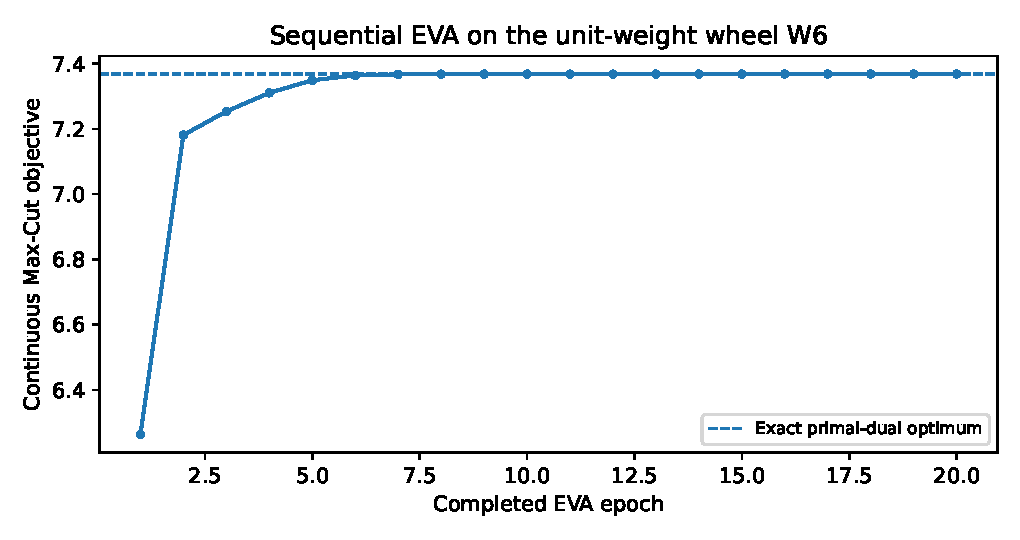
\includegraphics[width=.82\textwidth]{figures/eva_wheel6_trace.pdf}
\caption{An independently regenerated trace of sequential coordinate-ascent EVA on $W_6(1)$ (seed 2026, rank 4); the dashed horizontal line is the analytically certified SDP optimum.}\label{fig:eva-trace}
\end{figure}

\section{Full objective, Gram error, and cut error are different diagnostics}
A small primal objective error does not force the embedding to be close to a unique matrix, since optima may not be unique. The Frobenius discrepancy $\norm{YY^\top-X^*}_F$ is meaningful relative to a specified reference Gram matrix and is rotation invariant. The final rounded cut is a separate random or deterministic object; its value is at most $7$ even when the continuous objective is approximately $7.368$.

\section{An example of rounder quality versus relaxation quality}
For the wheel's exact three-dimensional Gram solution at $q=1$, each rim edge has
\[
X_{i,i+1}=-c+(1+c)(a^*)^2\approx-0.6708203933,
\]
while each spoke has $X_{i,5}=-a^*\approx-0.2763932023$. By the random-hyperplane formula,
\begin{align}
\E[\Cut(x)]&=\frac5\pi\arccos(-0.6708203933)+\frac5\pi\arccos(-0.2763932023)\\
&\approx 6.6159853305.
\end{align}
The theoretical cut optimum is $7$. A strong discrete result can therefore be obtained by selecting the best of several hyperplane samples or applying local improvement after rounding, even though the SDP matrix remains fixed. This is precisely why separating \emph{continuous optimization quality} from \emph{rounding quality} matters.

\chapter{Reproducing the SDP--EVA--Factorization Comparison}\label{ch:reproduce}
\section{Two programs, one graph, two different optimizations}
The comparison is between (A) a convex conic problem in $X$, and (B) a nonconvex product-of-spheres problem in $Y$. A fair investigation must score both using the same graph and $F(X)=\tr(LX)/4$, then apply the same rounding methods separately to each factor. The included script \texttt{code/solve\_sdp\_compare.py} implements both routes for $C_5$ and $W_6(1)$; it uses CVXPY if installed. The independent \texttt{code/check\_examples.py} requires only NumPy and verifies the analytic primal and dual constructions without a conic solver.

\section{Primal SDP in CVXPY}
The essential CVXPY model is:
\begin{lstlisting}[style=py]
import cvxpy as cp
X = cp.Variable((n, n), symmetric=True)
problem = cp.Problem(
    cp.Maximize(cp.trace(L @ X) / 4.0),
    [cp.diag(X) == 1.0, X >> 0]
)
problem.solve(solver=cp.SCS, eps=1e-7, max_iters=50000)
\end{lstlisting}
The \texttt{>>} constraint denotes PSD, not elementwise nonnegativity. The objective is linear in $X$. CVXPY is a modeling environment: \texttt{SCS}, \texttt{SDPA}, or another installed conic solver performs the numerical optimization. A solver status alone cannot certify accuracy to arbitrary precision.

\section{Factorization after CVXPY}
The source code uses spectral decomposition of the symmetrized numerical matrix and explicitly reports negative eigenvalues:
\begin{lstlisting}[style=py]
S = (Xvalue + Xvalue.T) / 2
lamb, Q = np.linalg.eigh(S)
if lamb.min() < -1e-5:
    raise ValueError("Unacceptable PSD violation")
V = Q * np.sqrt(np.maximum(lamb, 0))[None, :]
V /= np.linalg.norm(V, axis=1, keepdims=True)
\end{lstlisting}
This is a spectral square root, not Cholesky. For exact singular matrices, the spectral factorization is appropriate; the rank can be reduced by discarding exact or controlled near-zero eigenvalues. Renormalizing rows changes the resulting Gram matrix when the solver's diagonal is not exactly one, and the change must be disclosed.

\section{EVA without forming a dense Gram matrix}
The core update is:
\begin{lstlisting}[style=py]
for i in range(n):
    h = W[i] @ Y
    s = np.linalg.norm(h)
    if s > 1e-14:
        Y[i] = -h / s  # sequential, in place
\end{lstlisting}
For large sparse graphs, use CSR adjacency lists to avoid a dense $W$. To score a continuous candidate without constructing $YY^\top$, sum only the dot products on actual edges:
\begin{lstlisting}[style=py]
value = 0.5 * sum(
    weight * (1 - np.dot(Y[i], Y[j]))
    for i, j, weight in edges
)
\end{lstlisting}
The exact per-update gain can be verified against \eqref{eq:eva-gain} in a unit test.

\section{Independent dual validation}
For a candidate $Y$ in an approximate EVA fixed point, compute $h_i=\sum_jw_{ij}y_j$, $s_i=\norm{h_i}$, $\nu_i=(d_i+s_i)/4$, and $Z=\Diag(\nu)-L/4$. Check $\lambda_{\min}(Z)$ and $\norm{ZY}_F$. In the known analytic examples, the exact $X^*$ and $Z^*$ constructed in earlier chapters satisfy $\lambda_{\min}(X^*)\ge0$, $\lambda_{\min}(Z^*)\ge0$ and $Z^*X^*=0$. For an approximate run, use numerical bounds and report precision rather than calling near-zero numbers exact zeros.

\section{Recommended reproducibility commands}
\begin{lstlisting}[style=py]
# From the folder containing main.tex:
# python -m pip install numpy scipy
python code/check_examples.py

# Optional independent convex numerical solve:
# python -m pip install cvxpy scs
python code/solve_sdp_compare.py

# Compile and preserve an auditable artifact:
# latexmk -pdf -interaction=nonstopmode -halt-on-error main.tex
\end{lstlisting}
The printed values are numerical diagnostics and should be contrasted with the exact formulas \eqref{eq:c5cert} and \eqref{eq:wheel-optimal}. The project deliberately includes no dependency on the original university VM's already archived EVA factors; these analytic toy instances are distinct independent demonstrations.

\chapter{Experimental Design, Failure Modes, and Research Questions}\label{ch:protocol}
\section{Three independent layers of evaluation}
\paragraph{Layer I: continuous optimization.} For a fixed graph, compare the original signed-weight input hash, $F(Y_{\mathrm{EVA}})$, $F(X_{\mathrm{CVX}})$, primal feasibility, dual feasibility, the SDP upper bound, memory, runtime, rank and convergence diagnostics. If a numerical convex solver returns a lower primal objective than an EVA feasible candidate, report the discrepancy and seek improved accuracy rather than asserting that the convex optimum is smaller.

\paragraph{Layer II: Gram geometry.} Compare $\norm{Y_{\mathrm{EVA}}Y_{\mathrm{EVA}}^\top-X_{\mathrm{CVX}}}_F$, spectrum, effective rank, selected edge cosines and distances, and row norm errors. Two factors can have different coordinates but the same Gram matrix due to right orthogonal transformations. For large $n$, compute edgewise discrepancies or randomized trace estimates without materializing a dense $n\times n$ matrix.

\paragraph{Layer III: rounding.} Fix one factor, pair seeds, run GW and every clustering/refinement method under the same evaluation budget, and score the original graph objective. Save the best observed \emph{discrete} cut at every meaningful iteration, not merely the final iterate. Compare rounders on the \emph{same factor} to isolate rounding effects. If the factor changes, report a distinct two-factor experiment rather than a pure rounding comparison.

\section{Statistical sampling and uncertainty}
For $R$ random roundings with scores $c_1,\ldots,c_R$, estimate $\overline c=R^{-1}\sum_rc_r$ and sample variance $s_c^2=(R-1)^{-1}\sum_r(c_r-\overline c)^2$. Report means and distributions alongside best-of-$R$ cuts: best-of-$R$ is an order statistic and increases in expectation with $R$, so comparisons require matched restart counts. With paired seeds, calculate differences $d_r=c_r^{(A)}-c_r^{(B)}$ to reduce between-seed variance. Graphwise aggregates should use a declared weighting (equal graph or equal edge mass), and multiple-comparison uncertainty should not be confused with descriptive rankings.

\section{Numerical precision and stopping criteria}
An EVA angular tolerance, a convex solver's primal residual tolerance, and the absolute duality gap are not interchangeable. For EVA, report $\max\theta_{t,i}$, $\norm{\operatorname{grad}F(Y)}_F$, $\lambda_{\min}(Z)$, and the completed sweep count. For the convex solver, report the primal residual, minimal eigenvalue and whether a feasible dual objective was independently validated. If PSD projection is used, score both pre- and postrepair matrices and disclose the repair threshold.

\section{Research hypotheses worth testing}
\begin{enumerate}
\item \emph{Rank and geometry:} does increasing $p$ toward the conservative $\Theta(\sqrt n)$ regime systematically improve EVA's primal objective, yet make rounding slower or less stable?
\item \emph{Certificate frequency:} on which graph families does the candidate dual slack from an EVA fixed point become PSD without additional optimization? Can a small diagonal shift produce informative near-optimal bounds?
\item \emph{Clustering versus random hyperplanes:} controlling for a common fixed embedding, which method yields the best expected cut, best-of-$R$ cut and variance?
\item \emph{Structure-dependent behavior:} do odd cycles, toroidal instances, signed edges, and highly heterogeneous degree distributions predict differences in EVA convergence or rounding performance?
\item \emph{Numerical equivalence:} when CVXPY and EVA report nearly equal continuous objectives, are their Gram matrices close, or are there substantially different optimal faces?
\end{enumerate}
Each hypothesis should be associated with a prespecified statistic, common graph identity, random seeds and a negative-result reporting rule.

\section{Repository-first preservation protocol}
Do not overwrite the project's existing experimental solutions or rerun expensive SDP/EVA optimizations for purely pedagogical comparisons. For a new research experiment, assign the next sequential \texttt{experimentNNN} identifier, preserve script, graph hash, environment versions, settings, numerical results, plots, notes and exact reproduction steps. Keep an \texttt{AGENTS.md} or handoff note current, and push changes to a scoped branch for review without merging unless authorized. Large factor files should use repository-approved storage or Git LFS with verified remote backup. This monograph's \texttt{experiments/experiment001} is a standalone pedagogical verification campaign, not a renumbering of the existing maxkcut repository's experiments.

\appendix
\chapter{Supplementary Proofs, Extensions, and Common Misconceptions}\label{app:proofs}
\section{The complete graph $K_4$ shows nonuniqueness of SDP solutions}
For the unweighted complete graph on four vertices, the discrete best cut is $4$. One rank-one optimum is $x=(1,1,-1,-1)^\top$ and $X_1=xx^\top$. A different optimal Gram matrix is $X_2=(4/3)I_4-(1/3)\one\one^\top$, with ones on the diagonal, $-1/3$ off diagonal, and eigenvalues $(0,4/3,4/3,4/3)$. Both have objective $4$. The equality follows from
\[
F(X)=3-\frac12\sum_{i<j}X_{ij},\qquad \one^\top X\one=4+2\sum_{i<j}X_{ij}\ge0.
\]
Thus $F(X)\le4$, with both $X_1$ and $X_2$ attaining equality. A CVXPY solver and a factorized solver can therefore return different optimal Gram matrices, not merely differently rotated copies of one matrix.

\section{Why maximizing the Frobenius norm is a different problem}
For any rank-one cut matrix $X=xx^\top$ with $x_i=\pm1$, $\norm{X}_F^2=\tr(X^2)=\tr(nxx^\top)=n^2$, so $\norm{X}_F=n$ independent of the cut's weight. For the $K_4$ example, two very different cuts have the same Frobenius norm $4$ but different objectives. Hence $\max\norm{X}_F$ is not Max-Cut, even under unit diagonal and PSD constraints.

\section{Generalization to Max-$k$-Cut}
The Frieze--Jerrum relaxation uses a regular simplex encoding for $k$ groups. Its Gram constraints are
\[
X\succeq0,\quad X_{ii}=1,\quad X_{ij}\ge-\frac1{k-1},
\]
and its cut objective can be written $\frac{k-1}{2k}\ip{L}{X}$. For $k=2$, the lower bound $-1$ is already implied by PSD and unit diagonals, and the coefficient reduces to $1/4$. For $k>2$, the off-diagonal lower bounds are essential. \emph{The EVA algorithm studied in this monograph implements the $k=2$ vector relaxation}; merely supplying $k>2$ to the objective does not enforce the additional constraints. A general Max-$k$-Cut factorized solver needs a separate feasibility-preserving mechanism.

\section{A direct test of spectral factorization}
If $X$ is exactly PSD and $\diag X=\one$, let $X=Q\Lambda Q^\top$ and $Y=Q\Lambda^{1/2}$. Then $YY^\top=X$, each row has length one, and $F(Y)=F(X)$. For the same matrix, any orthogonal transformation $YR$ produces identical Gram entries and therefore the same probability law of isotropic Gaussian-hyperplane rounding. Cholesky and eigen factors are just different coordinate representations when both are exact.

\section{A tight gap identity}
For any primal feasible $X$ and dual feasible $\nu$, the primal--dual gap is
\[
\mathrm{Gap}(X,\nu)=\sum_i\nu_i-\frac14\ip{L}{X}=\ip{Z}{X}\ge0.
\]
If $X=YY^\top$, this becomes $\mathrm{Gap}=\tr(Y^\top ZY)=\norm{Z^{1/2}Y}_F^2$. This explains why complementarity $ZY=0$ gives zero gap. It also shows why no amount of Cholesky factorization, by itself, reduces the gap of a fixed primal matrix.

\section{What to remember}
\begin{takeaway}
\[
\boxed{
\begin{gathered}
\text{choose feasible }X\ \text{or unit-row }Y;\qquad X=YY^\top;\\
F(X)=\frac14\ip{L}{X}=\frac12\sum_{\{i,j\}\in E}w_{ij}(1-X_{ij});\\
\text{EVA: }y_i\gets-\frac{\sum_jw_{ij}y_j}{\norm{\sum_jw_{ij}y_j}};\qquad
\text{certificate: }Z=\Diag(\nu)-L/4\succeq0,\ ZY=0.
\end{gathered}}
\]
\end{takeaway}

\backmatter
\begin{thebibliography}{99}
\addcontentsline{toc}{chapter}{References}
\bibitem{eva2026} B. Gonzalez-Torres, A. E. Rodriguez-Fernandez, R. Menchaca-Mendez, R. Menchaca-Mendez, and O. Sch\"utze, ``EVA: A fast greedy optimization algorithm for the max-cut vector relaxation problem,'' \emph{Results in Control and Optimization}, vol. 24, article 100759, 2026. \url{https://doi.org/10.1016/j.rico.2026.100759}.
\bibitem{gw1995} M. X. Goemans and D. P. Williamson, ``Improved approximation algorithms for maximum cut and satisfiability problems using semidefinite programming,'' \emph{Journal of the ACM}, vol. 42, no. 6, pp. 1115--1145, 1995. \url{https://doi.org/10.1145/227683.227684}.
\bibitem{burer2003} S. Burer and R. D. C. Monteiro, ``A nonlinear programming algorithm for solving semidefinite programs via low-rank factorization,'' \emph{Mathematical Programming}, vol. 95, pp. 329--357, 2003.
\bibitem{burer2005} S. Burer and R. D. C. Monteiro, ``Local minima and convergence in low-rank semidefinite programming,'' \emph{Mathematical Programming}, vol. 103, pp. 427--444, 2005.
\bibitem{boumal2016} N. Boumal, V. Voroninski, and A. S. Bandeira, ``The non-convex Burer--Monteiro approach works on smooth semidefinite programs,'' \emph{Advances in Neural Information Processing Systems}, vol. 29, 2016. \url{https://arxiv.org/abs/1606.04970}.
\bibitem{boumal2020} N. Boumal, V. Voroninski, and A. S. Bandeira, ``Deterministic guarantees for Burer--Monteiro factorizations of smooth semidefinite programs,'' \emph{Communications on Pure and Applied Mathematics}, 2020. \url{https://arxiv.org/abs/1804.02008}.
\bibitem{waldspurger2020} I. Waldspurger and A. Waters, ``Rank optimality for the Burer--Monteiro heuristic,'' \emph{SIAM Journal on Optimization}, vol. 30, no. 3, pp. 2577--2602, 2020.
\bibitem{pataki1998} G. Pataki, ``On the rank of extreme matrices in semidefinite programs and the multiplicity of optimal eigenvalues,'' \emph{Mathematics of Operations Research}, vol. 23, no. 2, pp. 339--358, 1998.
\bibitem{vandenberghe1996} L. Vandenberghe and S. Boyd, ``Semidefinite programming,'' \emph{SIAM Review}, vol. 38, no. 1, pp. 49--95, 1996.
\bibitem{rodriguez2020} A. E. Rodriguez-Fernandez, B. Gonzalez-Torres, R. Menchaca-Mendez, and P. F. Stadler, ``Clustering improves the Goemans--Williamson approximation for the Max-Cut problem,'' \emph{Computation}, vol. 8, no. 3, article 75, 2020. \url{https://doi.org/10.3390/computation8030075}.
\bibitem{rodriguez2021} A. E. Rodriguez Fernandez, \emph{On the Study of Fitness Landscapes and the Max-Cut Problem}, doctoral dissertation, Universit\"at Leipzig, 2021. Provided project reference document.
\bibitem{felzenszwalb2022} P. Felzenszwalb, C. Klivans, and A. Paul, ``Clustering with semidefinite programming and fixed point iteration,'' \emph{Journal of Machine Learning Research}, vol. 23, pp. 1--23, 2022. \url{https://jmlr.org/papers/v23/21-0402.html}.
\bibitem{cvxpy2016} S. Diamond and S. Boyd, ``CVXPY: A Python-embedded modeling language for convex optimization,'' \emph{Journal of Machine Learning Research}, vol. 17, pp. 1--5, 2016. \url{https://www.cvxpy.org/}.
\end{thebibliography}

\end{document}
